\documentclass[10pt,a4paper]{article}

\usepackage[utf8]{inputenc}
\usepackage[T1]{fontenc}
\usepackage{babel}
\usepackage[margin=1.6cm, top=1.4cm, bottom=1.4cm, headheight=14pt]{geometry}
\usepackage{xcolor}
\usepackage{enumitem}
\usepackage{titlesec}
\usepackage{fancyhdr}
\usepackage{graphicx}
\usepackage{tabularx}
\usepackage{booktabs}
\usepackage{microtype}
\usepackage{helvet}
\renewcommand{\familydefault}{\sfdefault}

\definecolor{accent}{RGB}{30, 80, 162}
\definecolor{muted}{RGB}{120, 120, 120}
\definecolor{rule}{RGB}{210, 215, 225}

\setlength{\parskip}{2pt}
\setlength{\parindent}{0pt}

% Header
\pagestyle{fancy}
\fancyhf{}
\fancyhead[L]{\small\color{muted} Système de Gestion de Flotte \enspace\textbar\enspace ADR Semaine 1}
\fancyhead[R]{\small\color{muted} 11 mars 2026}
\fancyfoot[C]{\small\color{muted}\thepage}
\renewcommand{\headrulewidth}{0pt}

% Sections : numéro en bleu + texte normal
\titleformat{\section}
  {\normalsize\bfseries\color{accent}}{}{0em}{}[\ \textcolor{rule}{\rule[0.5ex]{0.3\linewidth}{0.4pt}}]
\titlespacing{\section}{0pt}{10pt}{6pt}

\newcommand{\ruledline}{\textcolor{rule}{\rule{\linewidth}{0.4pt}}\vspace{4pt}}

\begin{document}


\begin{titlepage}
  \centering
  \vspace*{3cm}
  {\LARGE\bfseries UNIVERSITÉ DE ROUEN NORMANDIE\\[4pt]
  FACULTÉ DES SCIENCES ET TECHNIQUES\par}
  \vspace{2cm}
  {\large ANNÉE UNIVERSITAIRE 2025--2026\par}
  \vspace{2cm}
  \textcolor{rule}{\rule{\textwidth}{1.5pt}}
  \vspace{1cm}

  {\huge\bfseries\color{accent} Architecture Decision Records\par}
  \vspace{0.4cm}
  {\Large Système de Gestion de Flotte\par}
  \vspace{0.4cm}
  {\large Semaine 1\par}

  \vspace{1cm}
  \textcolor{rule}{\rule{\textwidth}{1.5pt}}
  \vfill
  {\small 11 mars 2026}
\end{titlepage}

\tableofcontents
\newpage

% ---- EN-TÊTE ----
{\fontsize{16}{20}\selectfont\bfseries\color{accent} Architecture Decision Records}\\[2pt]
{\large Système de Gestion de Flotte --- DHL Express}\\[4pt]
\ruledline
 
{\small Ce document recense les décisions d'architecture prises en semaine 1 pour le système de \textbf{suivi en temps réel de la flotte de véhicules DHL Express}. Le système couvre la gestion des livreurs, l'affectation des véhicules aux tournées, la maintenance du parc et les alertes automatiques. Les utilisateurs sont les \textbf{administrateurs}, \textbf{managers}, \textbf{techniciens} et \textbf{utilisateurs}.}
\vspace{4pt}
 
{\small\bfseries\color{accent} C1 --- Vue système}\\[4pt]
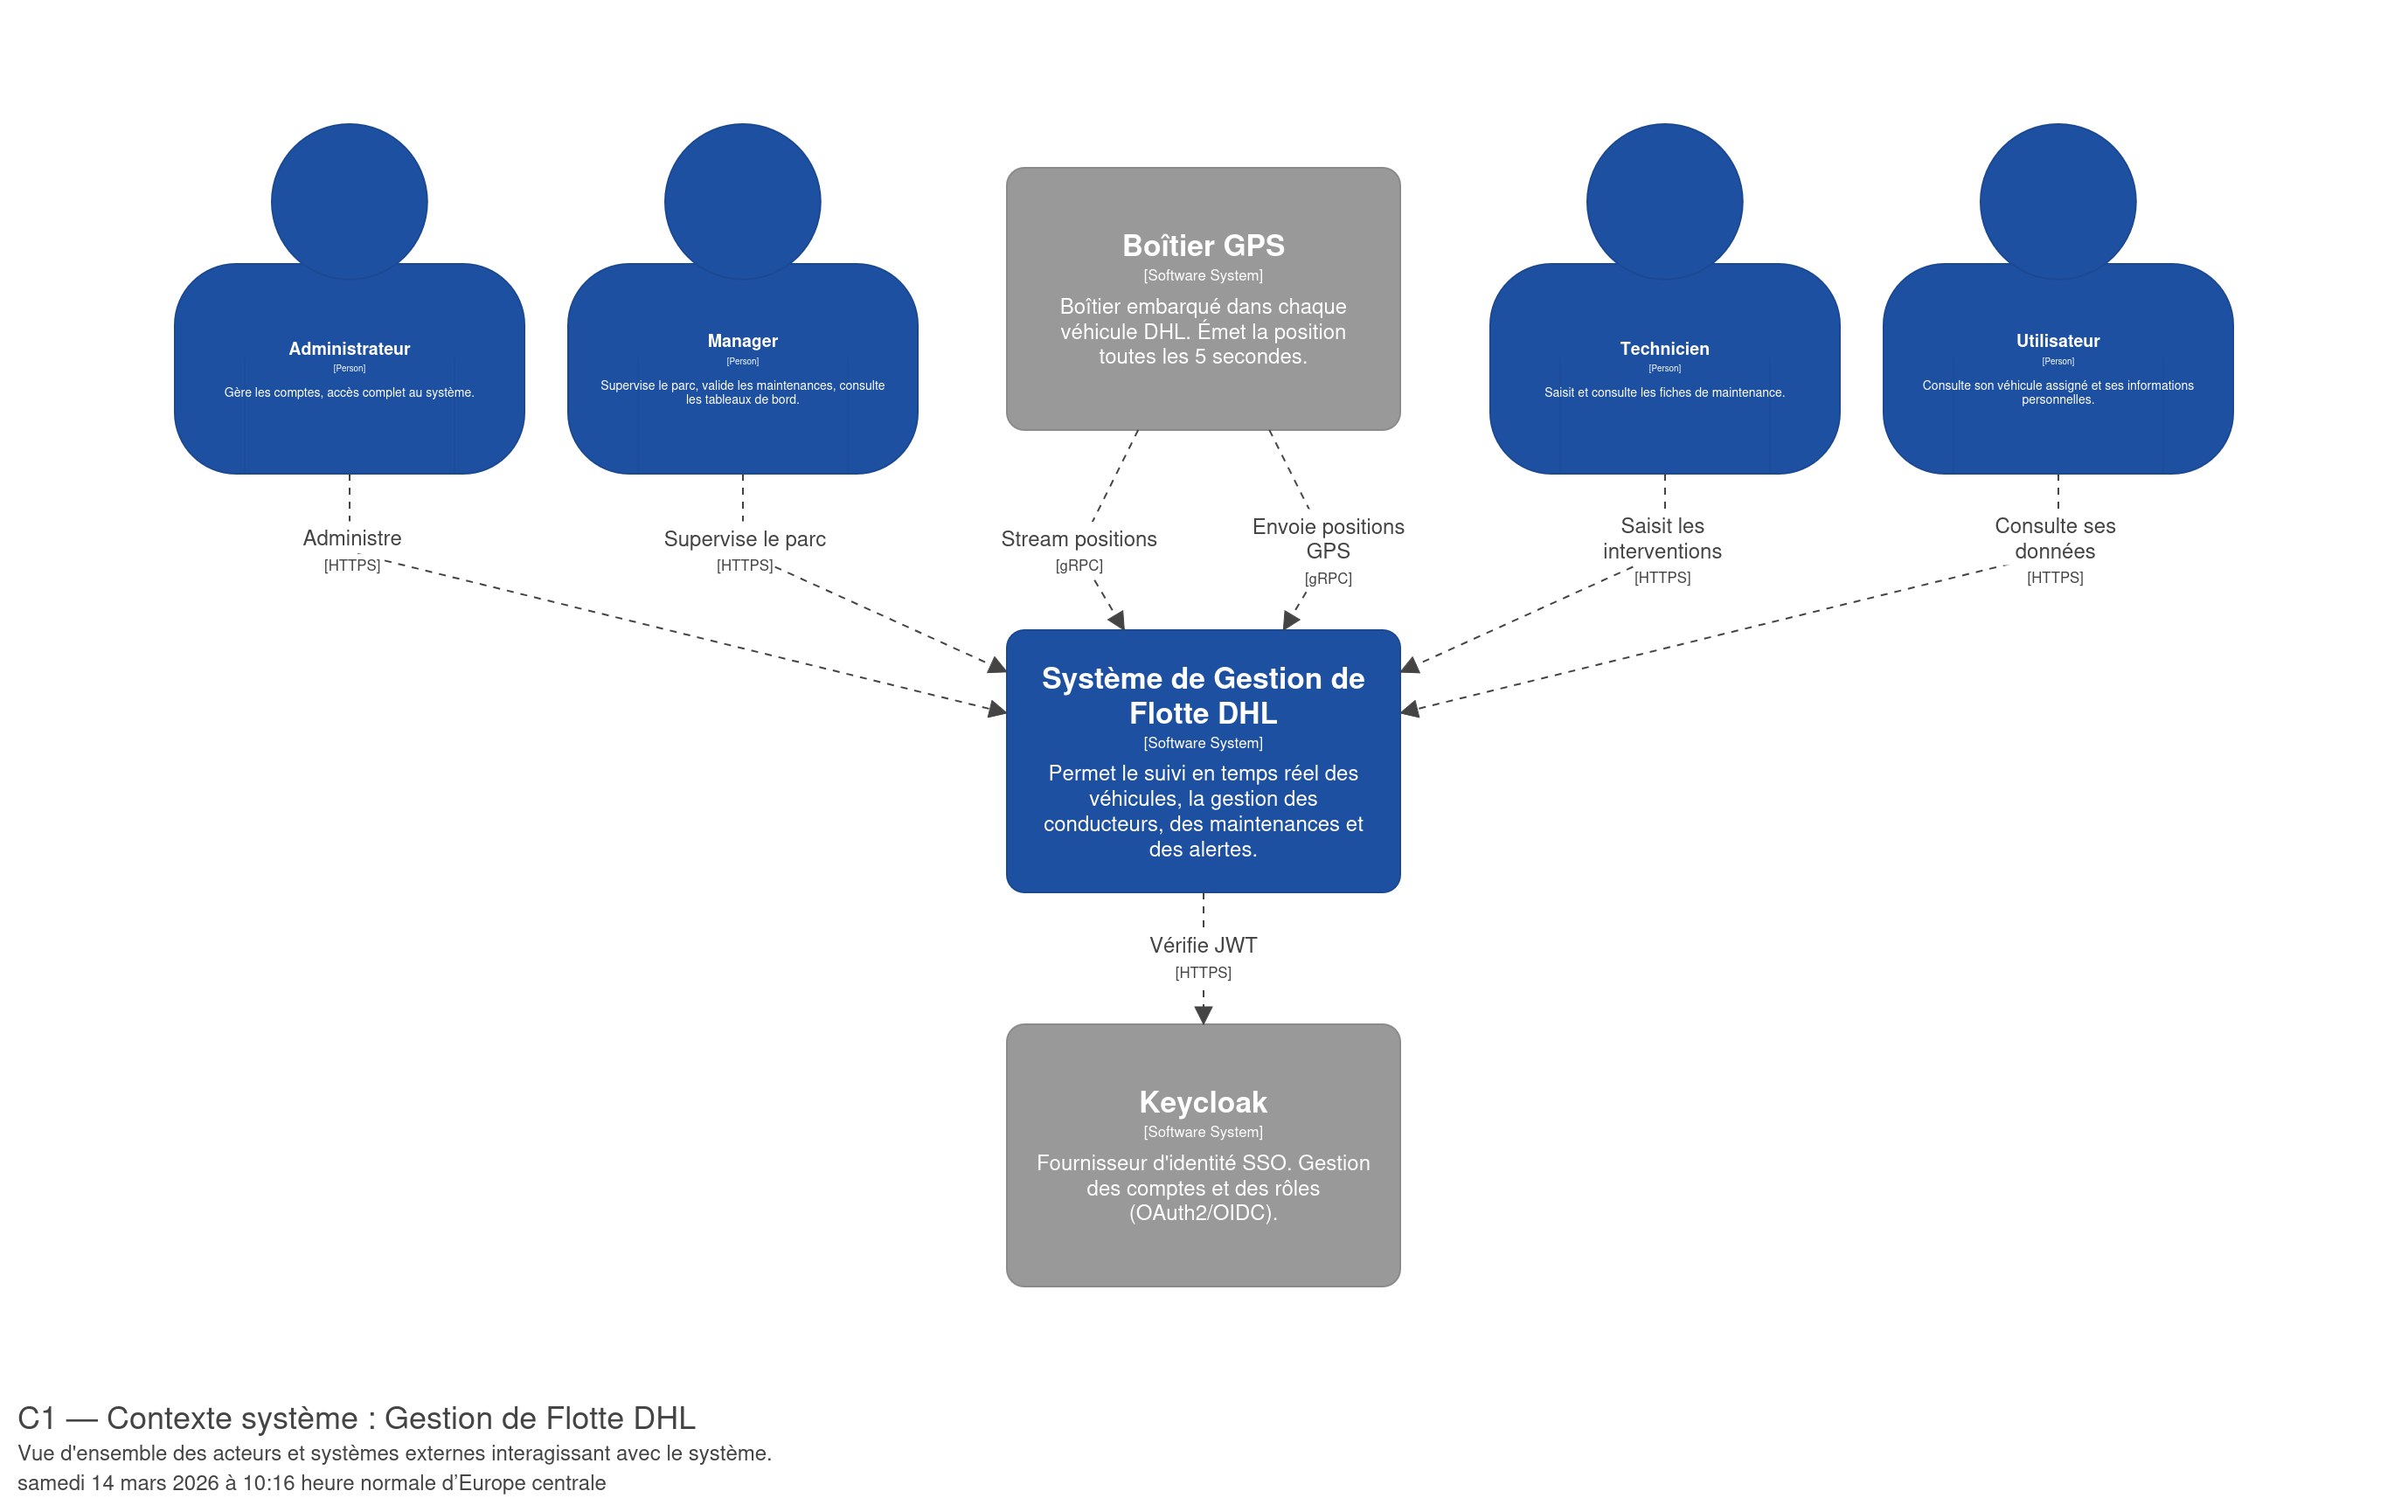
\includegraphics[width=\linewidth]{./C4/C1.png}
 
\vspace{10pt}
{\small\bfseries\color{accent} C2 --- Architecture des conteneurs}\\[4pt]
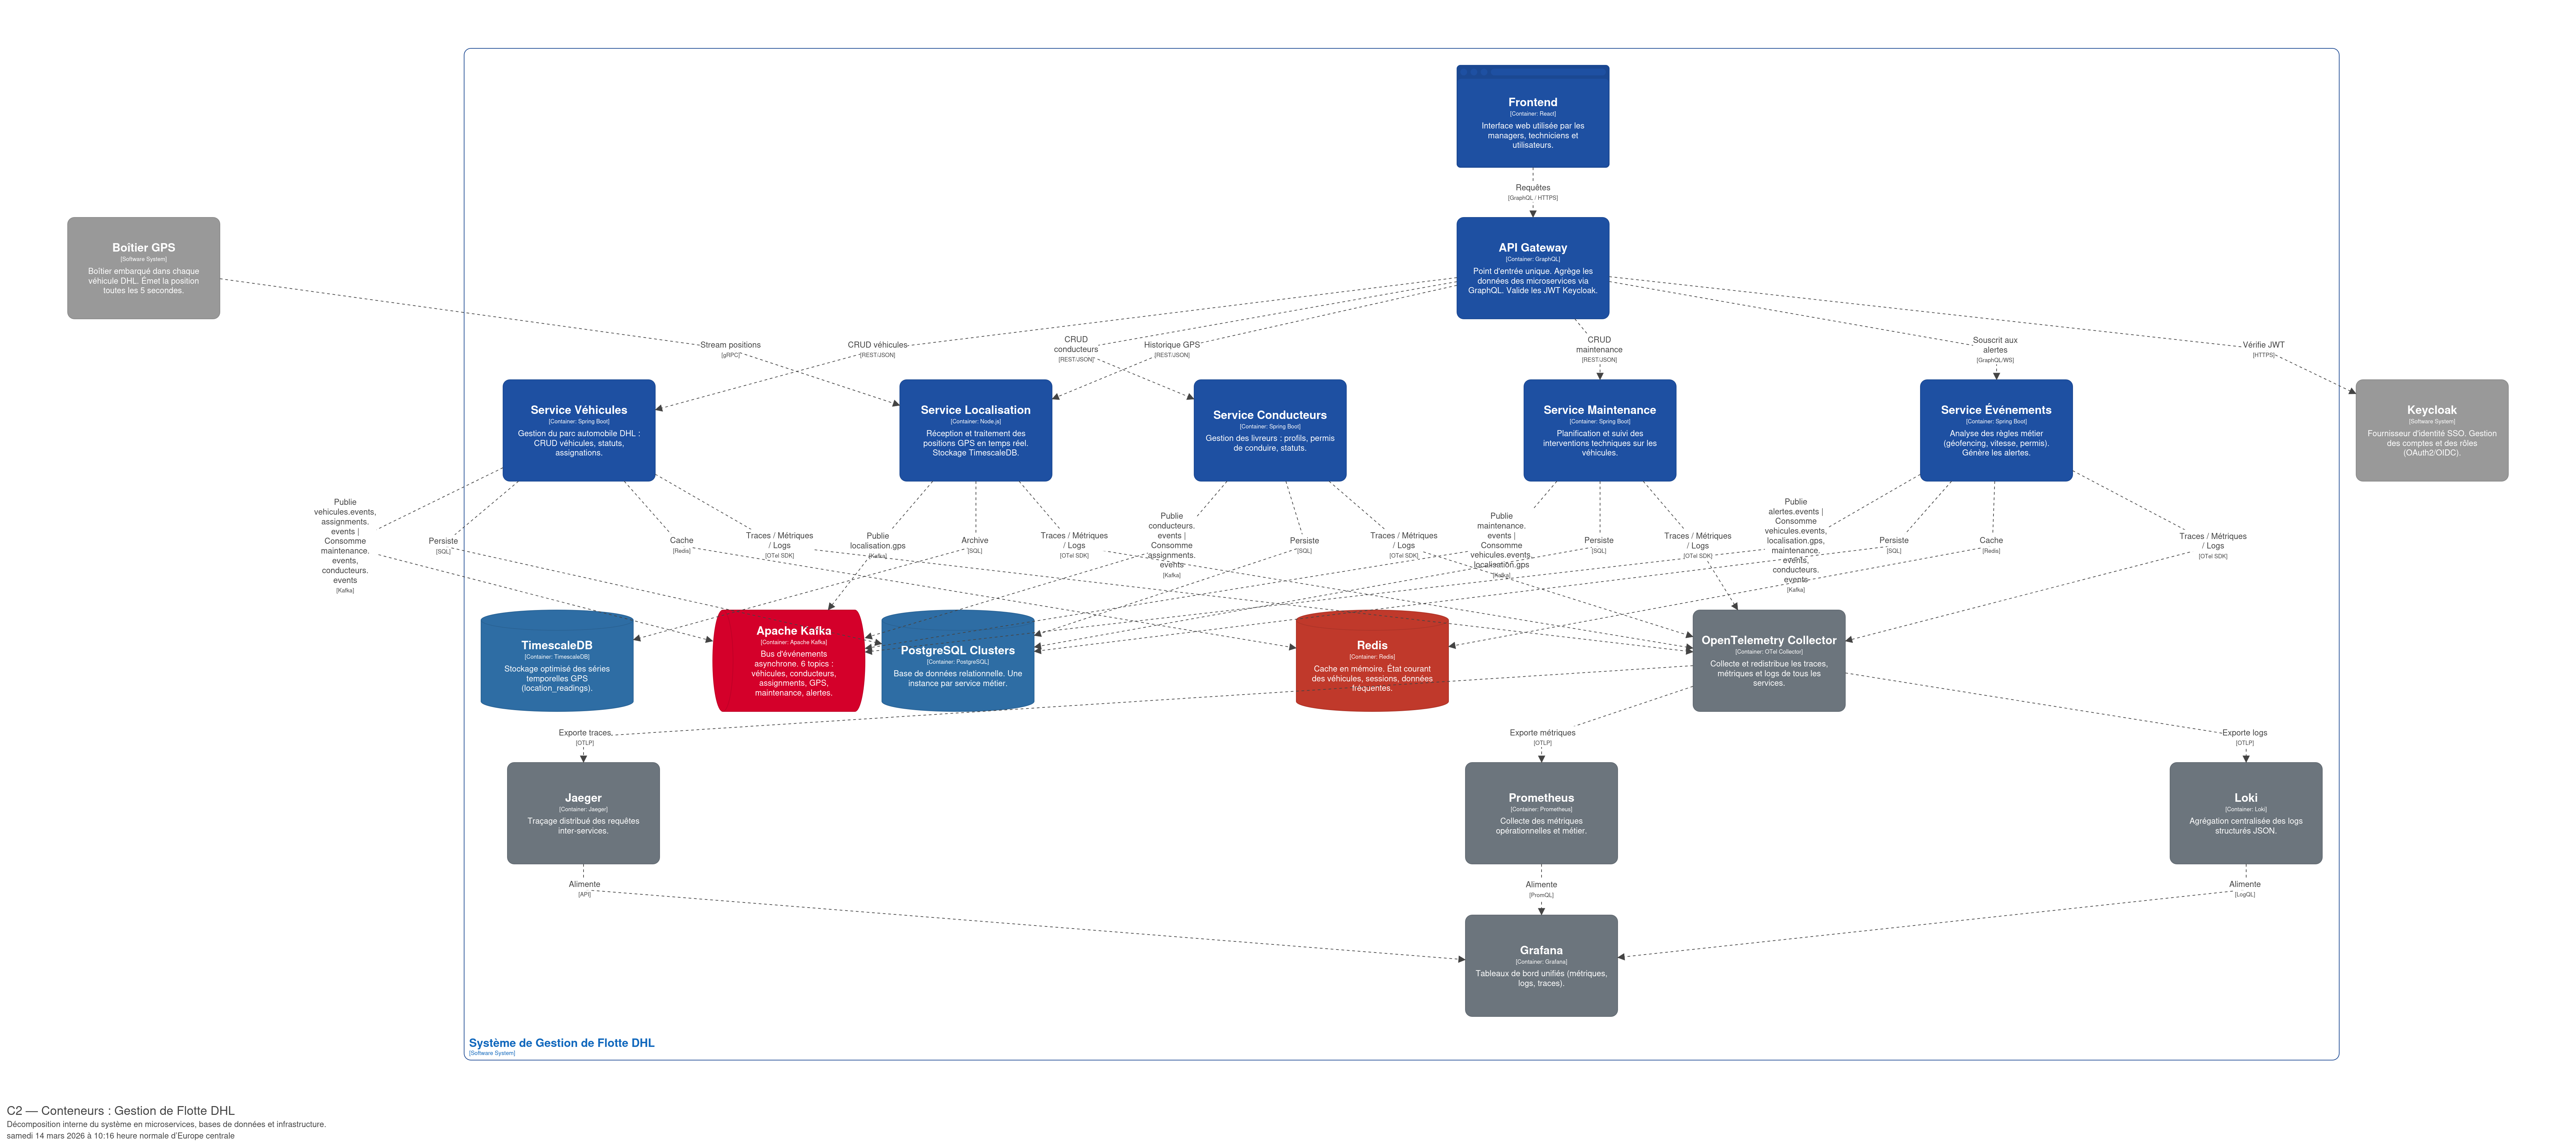
\includegraphics[width=\linewidth]{./C4/C2.png}
 
\vspace{6pt}
\ruledline

% ---- ADR ----

\section{ADR-001 — Services indépendants}

Le système doit faire trois choses à la fois : suivre les véhicules en direct, gérer les données administratives et envoyer des alertes. Ces trois besoins sont très différents et évolueront indépendamment.

\textbf{Décision :} séparer le système en trois parties indépendantes (Localisation, Administratif, Alertes), toutes accessibles depuis une seule adresse. \textbf{Avantage :} si une partie tombe en panne, les autres continuent de fonctionner. \textbf{Inconvénient :} un peu plus de choses à gérer au démarrage.



\section{ADR-002 — Protocole rapide pour le GPS}

Les boîtiers GPS envoient leur position plusieurs fois par seconde. Le protocole web classique n'est pas fait pour gérer autant de données en continu.

\textbf{Décision :} utiliser \textbf{gRPC}, un protocole conçu pour transmettre de grandes quantités de données rapidement. Les actions classiques (consulter, modifier) restent en HTTP normal. \textbf{Avantage :} les positions s'affichent sans délai perceptible. \textbf{Inconvénient :} une petite couche de traduction est nécessaire pour que le navigateur comprenne.



\section{ADR-003 — Alertes traitées sans bloquer le suivi}

Quand un véhicule dépasse une limite de vitesse ou entre dans une zone interdite, une alerte doit être envoyée. Cette étape ne doit pas ralentir le suivi GPS.

\textbf{Décision :} utiliser \textbf{Apache Kafka}, une file d'attente qui stocke les alertes à envoyer. Le suivi GPS dépose l'alerte, et le service d'envoi la traite quand il est prêt. \textbf{Avantage :} les deux parties travaillent sans se bloquer mutuellement, et aucune alerte n'est perdue. \textbf{Inconvénient :} un outil de plus à installer et surveiller.



\section{ADR-004 — Une base adaptée à chaque type de donnée}

Les positions GPS s'accumulent très rapidement, les données métier (véhicules, conducteurs) sont structurées et liées entre elles, et certaines informations sont consultées si souvent qu'elles doivent répondre en un instant.

\textbf{Décision :} utiliser trois bases de données, chacune adaptée à son rôle.

\begin{tabularx}{\linewidth}{lX}
  \toprule
  \small\textbf{Outil} & \small\textbf{Rôle} \\
  \midrule
  TimescaleDB  & Historique des positions GPS (conçu pour stocker efficacement des données qui arrivent en continu) \\
  PostgreSQL   & Véhicules, conducteurs, maintenances, alertes \\
  Redis        & Données consultées très souvent, stockées en mémoire pour répondre instantanément \\
  \bottomrule
\end{tabularx}



\section{ADR-005 — Connexion et droits centralisés}

Administrateurs, managers et techniciens n'ont pas accès aux mêmes fonctionnalités. Il faut un moyen simple de gérer qui peut faire quoi, sans le répéter dans chaque partie du système.

\textbf{Décision :} utiliser \textbf{Keycloak}, un outil gratuit qui centralise la gestion des comptes et des droits. L'utilisateur se connecte une seule fois et peut accéder à toutes les parties du système selon son rôle. \textbf{Avantage :} les droits sont gérés en un seul endroit. \textbf{Inconvénient :} si cet outil est en panne, plus personne ne peut se connecter — il doit donc toujours être disponible.

\vspace{3pt}
\ruledline


% ---- SCHEMAS BDD ----
{\small\color{muted} Schémas de base de données (PostgreSQL)}\\[4pt]
\begin{minipage}[t]{0.48\linewidth}
  \centering
  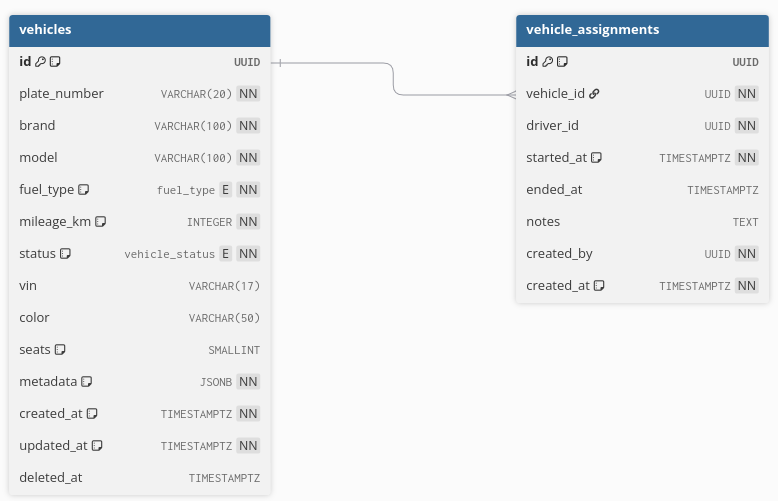
\includegraphics[width=0.75\linewidth]{./bd/b1.png}\\[4pt]
  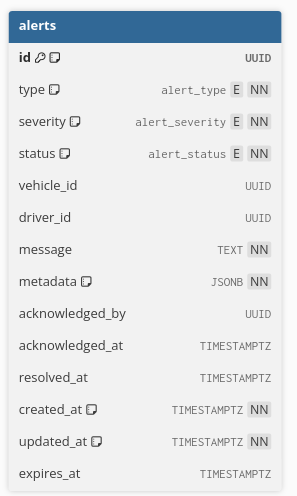
\includegraphics[width=0.75\linewidth]{./bd/b3.png}
\end{minipage}
\hfill
\begin{minipage}[t]{0.48\linewidth}
  \centering
  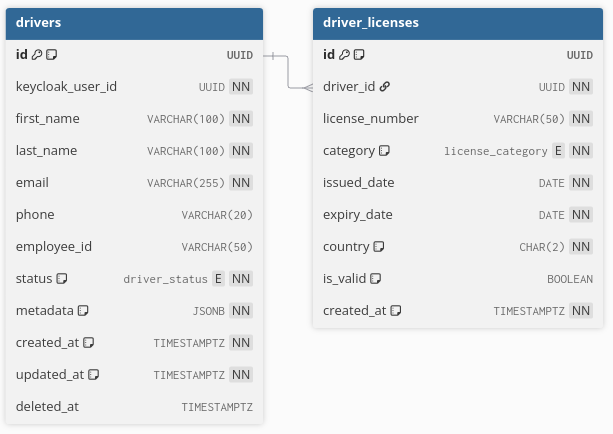
\includegraphics[width=0.75\linewidth]{./bd/b2.png}\\[4pt]
  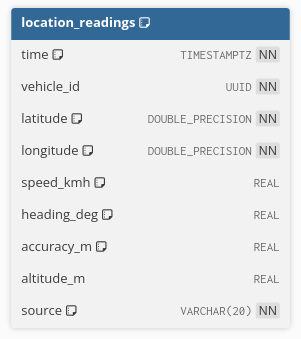
\includegraphics[width=0.75\linewidth]{./bd/b4.png}
\end{minipage}

\section{ADR-006 - Keycloak}

\newpage
 
% ================================================================
\section{Configuration Keycloak --- Semaine 1}
 
Cette section documente les étapes de mise en place de Keycloak réalisées en semaine 1, constituant le livrable de sécurité du projet.
 
% ---- 1. Déploiement ----
\subsection{1. Déploiement du serveur Keycloak en local}
 
Pour l'environnement de développement, Keycloak a été conteneurisé et lancé via Docker avec la création automatique d'un compte super-administrateur. La commande suivante démarre Keycloak en mode développement sur le port 8080 :
 
\begin{verbatim}
docker run -p 8080:8080
  -e KEYCLOAK_ADMIN=admin
  -e KEYCLOAK_ADMIN_PASSWORD=admin
  quay.io/keycloak/keycloak:latest start-dev
\end{verbatim}
 
L'interface d'administration est ensuite accessible sur \texttt{http://localhost:8080}.
 
% ---- 2. Realm ----
\subsection{2. Création du Realm}
 
Afin d'isoler notre environnement du realm \texttt{master} (réservé à l'administration de l'outil), un nouveau Realm dédié au projet a été créé :
 
\begin{itemize}[noitemsep]
  \item \textbf{Nom du Realm :} \texttt{gestion-flotte}
\end{itemize}
 
% ---- 3. Rôles RBAC ----
\subsection{3. Mise en place du contrôle d'accès (RBAC)}
 
Les rôles métier suivants ont été définis dans la section \textit{Realm roles} :
 
\vspace{4pt}
\begin{tabularx}{\linewidth}{lX}
  \toprule
  \small\textbf{Rôle} & \small\textbf{Périmètre} \\
  \midrule
  \texttt{admin}       & Accès complet à tous les services et données \\
  \texttt{manager}     & Supervision du parc, validation des maintenances \\
  \texttt{technicien}  & Lecture/écriture sur les fiches de maintenance \\
  \texttt{user}        & Consultation de ses propres données uniquement \\
  \bottomrule
\end{tabularx}
 
\vspace{6pt}
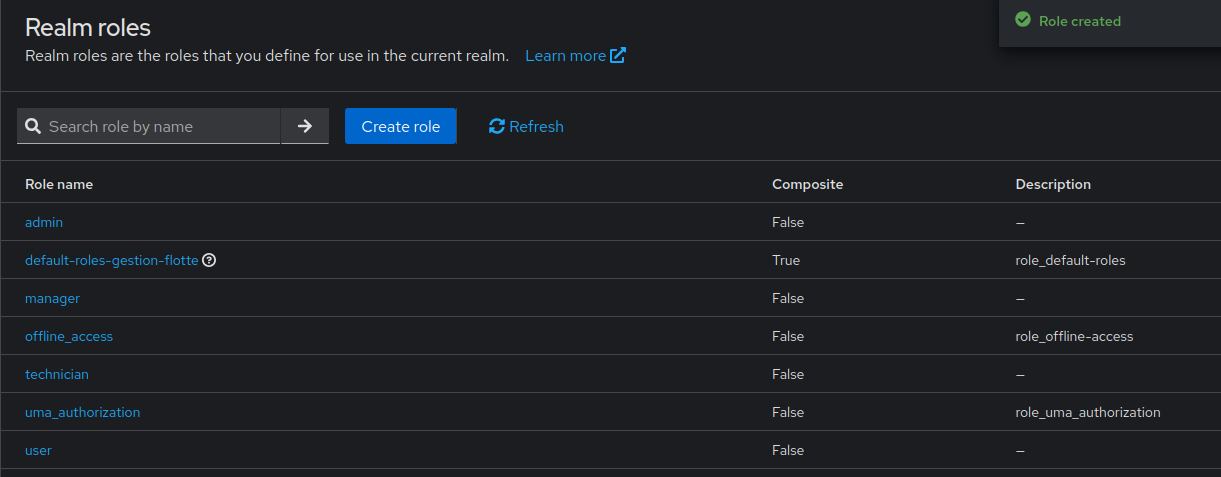
\includegraphics[width=\linewidth]{./keycloak/k2.png}\\
{\tiny\color{muted} Liste des Realm roles créés dans le realm \texttt{gestion-flotte}}
 
% ---- 4. Clients ----
\subsection{4. Configuration des Clients}
 
Deux clients ont été configurés pour interagir avec Keycloak :
 
\textbf{Client 1 : \texttt{frontend-web} (Client Public)} --- Destiné à l'interface React/Vue. Configuration : Standard flow activé, redirection autorisée vers \texttt{*} pour le développement.
 
\vspace{4pt}
\textbf{Client 2 : \texttt{api-gateway} (Client Confidentiel)} --- Destiné à la communication serveur à serveur. Configuration : \textit{Client authentication} activée, \textit{Service accounts roles} activés, génération d'un \textit{Client Secret} pour sécuriser les échanges GraphQL.
 
\vspace{6pt}
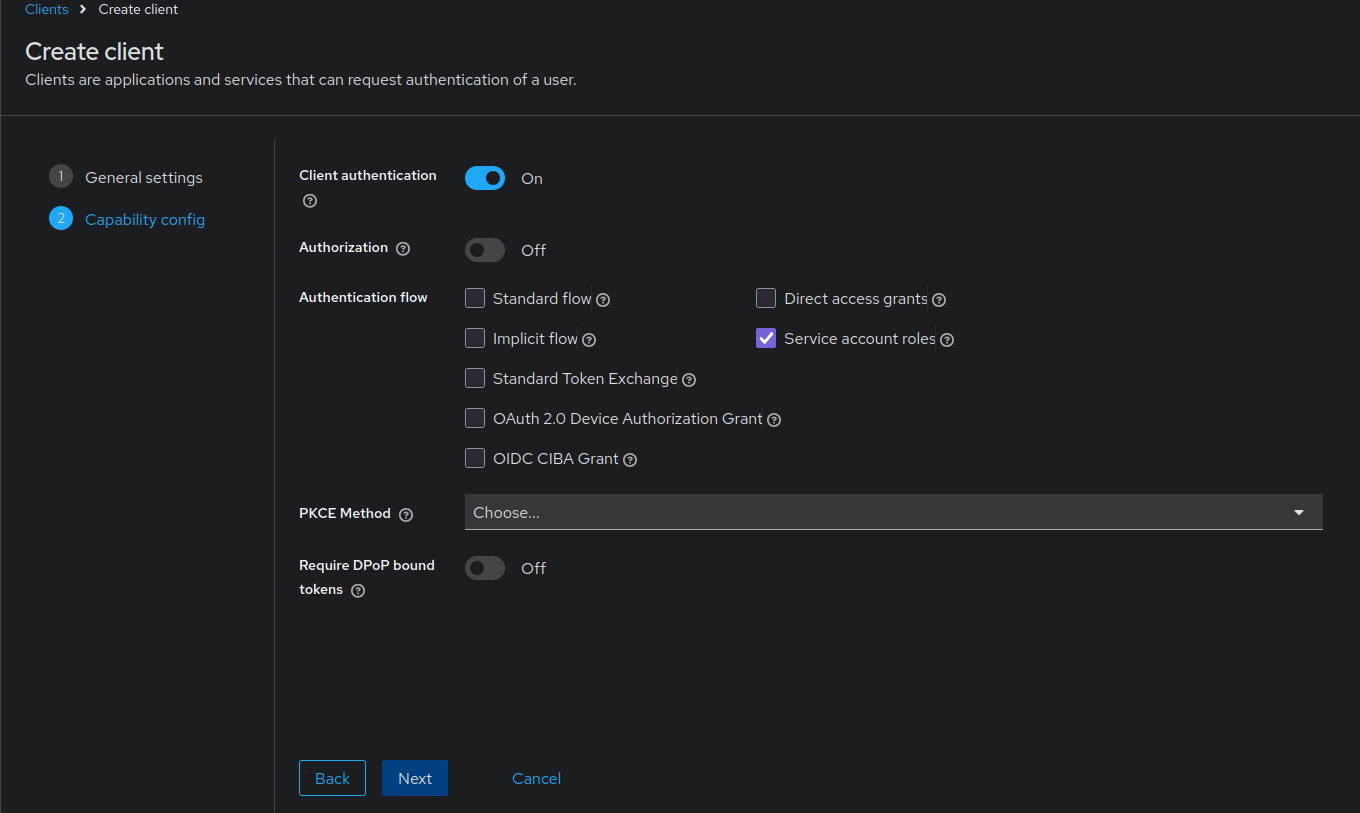
\includegraphics[width=\linewidth]{./keycloak/k1.png}\\
{\tiny\color{muted} Liste des clients configurés dans le realm \texttt{gestion-flotte}}
 
\vspace{8pt}
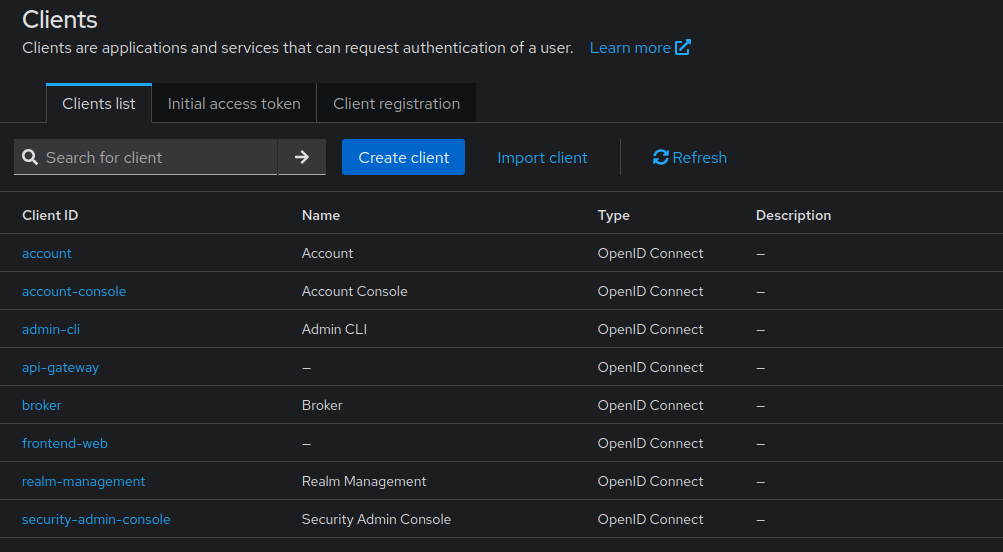
\includegraphics[width=0.75\linewidth]{./keycloak/k3.png}\\
{\tiny\color{muted} Configuration du client \texttt{api-gateway} --- Client authentication ON, Service account roles activé}
 
% ---- 5. Utilisateur de test ----
\subsection{5. Création d'un utilisateur de test}
 
Un utilisateur de test a été provisionné pour valider les futurs développements :
 
\vspace{4pt}
\begin{tabularx}{\linewidth}{lX}
  \toprule
  \small\textbf{Paramètre} & \small\textbf{Valeur} \\
  \midrule
  Identifiant   & \texttt{toto.admin} \\
  Mot de passe  & Défini manuellement, \textit{Temporary = OFF} \\
  Role mapping  & Rôle \texttt{admin} assigné \\
  \bottomrule
\end{tabularx}
 
\vspace{6pt}
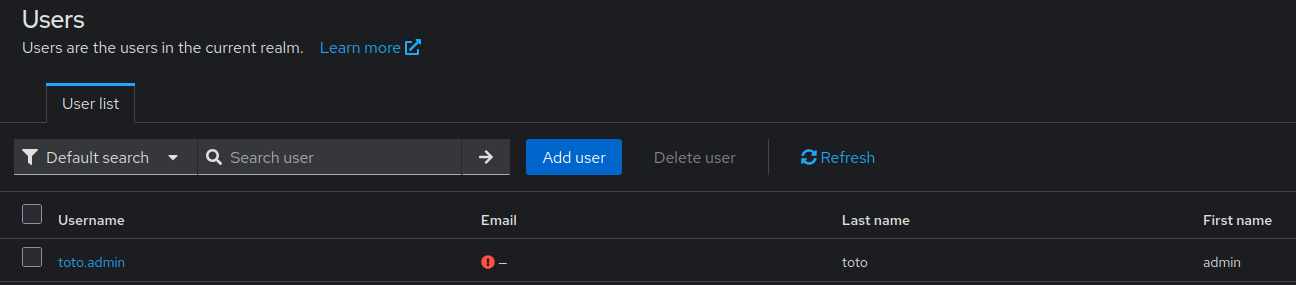
\includegraphics[width=\linewidth]{./keycloak/k4.png}\\
{\tiny\color{muted} Liste des utilisateurs du realm \texttt{gestion-flotte} --- utilisateur \texttt{toto.admin} créé avec le rôle \texttt{admin}}
 
% ---- 6. Export ----
\subsection{6. Exportation de la configuration (Livrable)}
 
Pour garantir la reproductibilité de l'environnement (\textit{Infrastructure as Code}), l'intégralité de la configuration a été exportée via l'interface Keycloak (Include clients + Include groups and roles). Le fichier généré \texttt{realm-export.json} est versionné dans le dépôt Git du projet sous le chemin \texttt{infrastructure/keycloak/realm-export.json}, ce qui permet de reconstruire l'environnement Keycloak complet automatiquement lors du déploiement en semaine 2.

\end{document}